% Figure: a path of three terms from Y to X and a sequence of sites along it. Transcription (for
% cheap agents): seven sites 0..6 on a line; the probe's region Y = {0, 1} (left box), the
% observable's region X = {5, 6} (right box); three supports drawn as rounded boxes above the
% line: S_{i_1} = {1, 2, 3}, S_{i_2} = {3, 4}, S_{i_3} = {4, 5}; the chosen sites u_0 = 1 (in
% S_{i_1} ∩ Y, on the boundary of Y), u_1 = 3 (in S_{i_1} ∩ S_{i_2}), u_2 = 4 (in S_{i_2} ∩ S_{i_3}),
% u_3 = 5 (in S_{i_3} ∩ X), marked by filled circles and joined by arrows labelled h_{13}, h_{34},
% h_{45}; the weights κ_{i_1} ≤ h_{13}, κ_{i_2} ≤ h_{34}, κ_{i_3} ≤ h_{45} written under the arrows.
% The label S_{i_3} sits above the box S_{i_3}, clear of the box S_{i_2}; the label u_3 sits
% slightly to the right of site 5, above the box of X, clear of S_{i_3}.
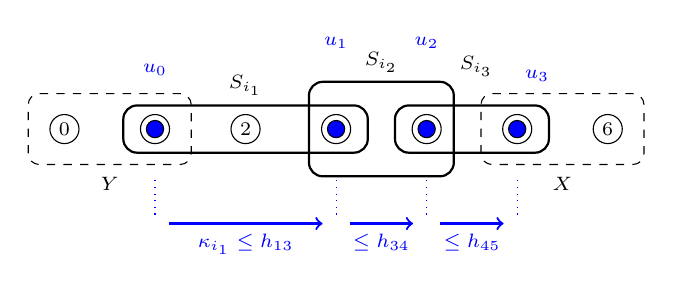
\begin{tikzpicture}[x=1.15cm,y=1cm,
  site/.style={circle,draw,fill=white,inner sep=1.6pt,font=\scriptsize},
  chosen/.style={circle,draw,fill=Blue,inner sep=2.2pt},
  edge/.style={rounded corners=5pt,draw,thick,fill=none},
  region/.style={rounded corners=4pt,draw,dashed,fill=none},
  lab/.style={font=\scriptsize}]
  % regions
  \draw[region] (-0.4,-0.45) rectangle (1.4,0.45);
  \node[lab] at (0.5,-0.7) {$Y$};
  \draw[region] (4.6,-0.45) rectangle (6.4,0.45);
  \node[lab] at (5.5,-0.7) {$X$};
  % supports
  \draw[edge] (0.65,-0.3) rectangle (3.35,0.3);   \node[lab] at (2,0.55) {$S_{i_1}$};
  \draw[edge] (2.7,-0.6) rectangle (4.3,0.6);     \node[lab] at (3.5,0.85) {$S_{i_2}$};
  \draw[edge] (3.65,-0.3) rectangle (5.35,0.3);   \node[lab] at (4.55,0.8) {$S_{i_3}$};
  % sites
  \foreach \s in {0,...,6} { \node[site] (s\s) at (\s,0) {\s}; }
  \node[chosen] at (1,0) {}; \node[chosen] at (3,0) {}; \node[chosen] at (4,0) {};
  \node[chosen] at (5,0) {};
  \node[lab,Blue] at (1,0.75) {$u_0$};
  \node[lab,Blue] at (3,1.1) {$u_1$};
  \node[lab,Blue] at (4,1.1) {$u_2$};
  \node[lab,Blue] at (5.22,0.68) {$u_3$};
  % the walk
  \draw[->,Blue,thick] (1.15,-1.2) -- (2.85,-1.2) node[midway,below,lab,Blue] {$\kappa_{i_1}\le h_{13}$};
  \draw[->,Blue,thick] (3.15,-1.2) -- (3.85,-1.2) node[midway,below,lab,Blue] {$\le h_{34}$};
  \draw[->,Blue,thick] (4.15,-1.2) -- (4.85,-1.2) node[midway,below,lab,Blue] {$\le h_{45}$};
  \foreach \s in {1,3,4,5} { \draw[Blue,dotted,thin] (\s,-0.65) -- (\s,-1.1); }
\end{tikzpicture}
